\newpage
\appendix
%%%%%%%%%%%%%%%%%%%%%%%%%%%%%%%%%%%%%%%%%%%%%%%%%%%%%%%%%%%%%%%%%%%%%%%%%%%%%%%%
%%%%%%%%%%%%%%%%%%%%%%%%%%%%%%%%%%%%%%%%%%%%%%%%%%%%%%%%%%%%%%%%%%%%%%%%%%%%%%%%
%%%%%%%%%%%%%%%%%%%%%%%%%%%%%%%%%%%%%%%%%%%%%%%%%%%%%%%%%%%%%%%%%%%%%%%%%%%%%%%%
\section{Physical Modelling}
\subsection{Circuit Analysis}\label{apx:circuit_analysis}
\subsubsection{$0 < t \leq d \cdot T$}
% First, the `on' period of the switching interval will be analysed. The relevant circuit in this instance is provided in Figure~\ref{cir:cuk_on}.
\begin{figure}[H]
\centering
\fbox{
\begin{circuitikz}[scale = 0.75]
\draw (0,0)
	to[V<=$v_g$, invert] (0,5)
	to[L, l=$L_1$, v_>=$v_{L1}$, i^>=$i_{L1}$] (3,5)
	to[R, l=$R_1$] (5,5)
	to[C, l=$C_1$, v_>=$v_{C1}$, i^>=$i_{C1}$] (8,5)
	to[R, l=$R_3$] (10,5)
	to[L, l=$L_2$, v_<=$v_{L2}$, i<^=$i_{L2}$] (13,5)
	to[R, l=$R_2$] (15,5)
	to[C, l_=$C_2$, v^<=$v_{C2}$, i<_=$i_{C2}$] (15,2)
	to[R, l=$R_4$] (15,0) -- (0,0);
\draw (5,5)
	to[R, l_=$R_o$] (5,0);
\draw (15,5) -- (18,5)
	to[R, l_=$R$] (18,0) -- (15,0);
\draw (18,5) -- (19,5);
\draw (18,0) -- (19,0);
\draw
	node[ocirc] (A)  at (19,5) {}
	node[ocirc] (B)  at (19,0) {}
	(A) to[open, v^>=$v_o$] (B);
\draw (18/2,0)
	node[ground] {};
\end{circuitikz}
}
\caption{}
\label{cir:cuk_on}
\end{figure}
~\\
\begin{align*}
i_{C2} = i_{L2} - i_R = i_{L2} - \frac{v_o}{R}
\qquad\text{and}\qquad
v_o = v_{C2} + v_{R4} = v_{C2} + i_{C2}R_4 = v_{C2} + \paren{i_{L2} - \frac{v_o}{R}}R_4
\end{align*}
\begin{align*}
\implies v_o &= v_{C2} \paren{\frac{R}{R + R_4}} + i_{L2} \paren{\frac{R \cdot R_4}{R + R_4}}
\end{align*}
\begingroup
\allowdisplaybreaks
\begin{align*}
\frac{\mathrm{d}v_{C1}}{\mathrm{d}t} &= \frac{i_{C1}}{C_1}\\[11pt]
&= \minus\frac{i_{L2}}{C_1}
\\[11pt]
\frac{\mathrm{d}v_{C2}}{\mathrm{d}t} &= \frac{i_{C2}}{C_2}\\[11pt]
&= \minus\frac{v_{C2} - i_{L2}R}{C_2 \paren{R + R_4}}
\\[11pt]
\frac{\mathrm{d}i_{L1}}{\mathrm{d}t} &= \frac{v_{L1}}{L_1}\\[11pt]
&= \frac{v_g - i_{L1}R_1 - (i_{L1} + i_{L2})R_o}{L_1}\\[11pt]
&= \frac{v_g - i_{L1}(R_1 + R_o) - i_{L2}R_o}{L_1}
\\[11pt]
\frac{\mathrm{d}i_{L2}}{\mathrm{d}t} &= \frac{v_{L2}}{L_2}\\[11pt]
&= \frac{\minus v_o + i_{L2}R_2 - (i_{L1} + i_{L2})R_o - v_{C1} - (\minus i_{L2}R_3)}{L_2}\\[11pt]
&= \frac{1}{L_2} \squarey{\minus \frac{v_{C2}R}{R + R_4} - \frac{i_{L2} R \cdot R_4}{R + R_4} + i_{L2}R_2 - (i_{L1} + i_{L2})R_o - v_{C1} + i_{L2}R_3}\\[11pt]
&= \frac{1}{L_2} \squarey{\minus v_{C1} - \frac{v_{C2}R}{R + R_4} - i_{L1}R_o + i_{L2} \paren{R_2 + R_3 - R_o - \frac{R \cdot R_4}{R + R_4}}}
\end{align*}
\endgroup
%%%%%%%%%%%%%%%%%%%%%%%%%%%%%%%%%%%%%%%%%%%%%%%%%%%%%%%%%%%%%%%%%%%%%%%%%%%%%%%%
~\\
~\rule{\textwidth}{0.5pt}
~\\
Per Equation~(\ref{eqn:equations_on}), the on-period matricies $\boldsymbol{A}_1$, $\boldsymbol{b}_1$, and $\boldsymbol{c}_1$ are thus populated as
\begin{align*}
\begin{bmatrix}
\dispdot{v_{C1}} \\ \dispdot{v_{C2}} \\ \dispdot{i_{L1}} \\ \dispdot{i_{L2}}
\end{bmatrix}
&=
\begin{bmatrix}
0 & 0 & 0 & \minus\frac{1}{C_1}\\
0 & \minus\frac{1}{C_2(R + R_4)} & 0 & \frac{R}{C_2(R + R_4)}\\
0 & 0 & \minus\frac{R_1 + R_o}{L_1} & \minus\frac{R_o}{L_1}\\
\minus\frac{1}{L_2} & \minus\frac{R}{L_2(R + R_4)} & \minus\frac{R_o}{L_2} & \frac{R_2 + R_3 - R_o - \frac{R \cdot R_4}{R + R_4}}{L_2}
\end{bmatrix}
\begin{bmatrix}
v_{C1} \\ v_{C2} \\ i_{L1} \\ i_{L2}
\end{bmatrix}
+
\begin{bmatrix}
0 & 0 & 0 & 0\\
0 & 0 & 0 & 0\\
\frac{1}{L_1} & 0 & 0 & 0\\
0 & 0 & 0 & 0
\end{bmatrix}
\begin{bmatrix}
v_g \\ V_D \\ 0 \\ 0
\end{bmatrix}
\\[11pt]
y &=
\begin{bmatrix}
0 & \frac{R}{R + R_4} & 0 & \frac{R \cdot R_4}{R + R_4}
\end{bmatrix}
\begin{bmatrix}
v_{C1} \\ v_{C2} \\ i_{L1} \\ i_{L2}
\end{bmatrix}
\end{align*}
%%%%%%%%%%%%%%%%%%%%%%%%%%%%%%%%%%%%%%%%%%%%%%%%%%%%%%%%%%%%%%%%%%%%%%%%%%%%%%%%
%%%%%%%%%%%%%%%%%%%%%%%%%%%%%%%%%%%%%%%%%%%%%%%%%%%%%%%%%%%%%%%%%%%%%%%%%%%%%%%%
\subsubsection{$d \cdot T < t \leq T$}
% Now the `off' period of the switching interval will be analysed. The relevant circuit in this instance is provided in Figure~\ref{cir:cuk_off}.
\begin{figure}[H]
\centering
\fbox{
\begin{circuitikz}[scale = 0.75]
\draw (0,0)
	to[V<=$v_g$, invert] (0,5)
	to[L, l=$L_1$, v_>=$v_{L1}$, i^>=$i_{L1}$] (3,5)
	to[R, l=$R_1$] (5,5)
	to[C, l=$C_1$, v_>=$v_{C1}$, i^>=$i_{C1}$] (8,5)
	to[R, l=$R_3$] (10,5)
	to[L, l=$L_2$, v_<=$v_{L2}$, i<^=$i_{L2}$] (13,5)
	to[R, l=$R_2$] (15,5)
	to[C, l_=$C_2$, v^<=$v_{C2}$, i<_=$i_{C2}$] (15,2)
	to[R, l=$R_4$] (15,0) -- (0,0);
\draw (15,5) -- (18,5)
	to[R, l_=$R$] (18,0) -- (15,0);
\draw (10,5)
	to[R, l_=$R_D$] (10,5/2)
	to[V_<=$V_D$] (10,0);
\draw (18,5) -- (19,5);
\draw (18,0) -- (19,0);
\draw
	node[ocirc] (A)  at (19,5) {}
	node[ocirc] (B)  at (19,0) {}
	(A) to[open, v^>=$v_o$] (B);
\draw (18/2,0)
	node[ground] {};
\end{circuitikz}
}
\caption{}
\label{cir:cuk_off}
\end{figure}
%
\begingroup
\allowdisplaybreaks
\begin{align*}
\frac{\mathrm{d}v_{C1}}{\mathrm{d}t} &= \frac{i_{C1}}{C_1}\\[11pt]
&= \frac{i_{L1}}{C_1}
\\[11pt]
\frac{\mathrm{d}v_{C2}}{\mathrm{d}t} &= \frac{i_{C2}}{C_2}\\[11pt]
&= \minus\frac{v_{C2} - i_{L2}R}{C_2 \paren{R + R_4}}
\\[11pt]
\frac{\mathrm{d}i_{L1}}{\mathrm{d}t} &= \frac{v_{L1}}{L_1}\\[11pt]
&= \frac{v_g - i_{L1}R_1 - v_{C1} - i_{L1}R_3 - (i_{L1} + i_{L2})R_D - V_D}{L_1}\\[11pt]
&= \frac{v_g - v_{C1} - i_{L1}(R_1 + R_3 + R_D) - i_{L2}R_D - V_D}{L_1}
\\[11pt]
\frac{\mathrm{d}i_{L2}}{\mathrm{d}t} &= \frac{v_{L2}}{L_2}\\[11pt]
&= \frac{\minus v_o + i_{L2}R_2 - V_D - (i_{L1} + i_{L2})R_D}{L_2}\\[11pt]
&= \frac{1}{L_2} \squarey{\minus \frac{v_{C2}R}{R + R_4} - \frac{i_{L2}R \cdot R4}{R + R_4} - i_{L1}R_D + i_{L2}(R_2 - R_D) - V_D}\\[11pt]
&= \frac{1}{L_2} \squarey{\minus \frac{v_{C2}R}{R + R_4} - i_{L1}R_D + i_{L2} \paren{R_2 - R_D - \frac{R \cdot R_4}{R + R_4}} - V_D}
\end{align*}
\endgroup
State space description:
\begin{align*}
\begin{bmatrix}
\dispdot{v_{C1}} \\ \dispdot{v_{C2}} \\ \dispdot{i_{L1}} \\ \dispdot{i_{L2}}
\end{bmatrix}
& =
\begin{bmatrix}
0 & 0 & \frac{1}{C_1} & 0\\
0 & \minus\frac{1}{C_2(R + R_4)} & 0 & \frac{R}{C_2(R + R_4)}\\
\minus\frac{1}{L_1} & 0 & \minus\frac{R_1 + R_3 + R_D}{L_1} & \minus\frac{R_D}{L_1}\\
0 & \minus\frac{R}{L_2(R + R_4)} & \minus\frac{R_D}{L_2} & \frac{R_2 - R_D - \frac{R \cdot R_4}{R + R_4}}{L_2}
\end{bmatrix}
\begin{bmatrix}
v_{C1} \\ v_{C2} \\ i_{L1} \\ i_{L2}
\end{bmatrix}
+
\begin{bmatrix}
0 & 0 & 0 & 0\\
0 & 0 & 0 & 0\\
\frac{1}{L_1} & {-}\frac{1}{L_1} & 0 & 0\\
0 & {-}\frac{1}{L_2} & 0 & 0
\end{bmatrix}
\begin{bmatrix}
v_g \\ V_D \\ 0 \\ 0
\end{bmatrix}
\\[11pt]
y &=
\begin{bmatrix}
0 & \frac{R}{R + R_4} & 0 & \frac{R \cdot R_4}{R + R_4}
\end{bmatrix}
\begin{bmatrix}
v_{C1} \\ v_{C2} \\ i_{L1} \\ i_{L2}
\end{bmatrix}
\end{align*}
%%%%%%%%%%%%%%%%%%%%%%%%%%%%%%%%%%%%%%%%%%%%%%%%%%%%%%%%%%%%%%%%%%%%%%%%%%%%%%%%
%%%%%%%%%%%%%%%%%%%%%%%%%%%%%%%%%%%%%%%%%%%%%%%%%%%%%%%%%%%%%%%%%%%%%%%%%%%%%%%%
%%%%%%%%%%%%%%%%%%%%%%%%%%%%%%%%%%%%%%%%%%%%%%%%%%%%%%%%%%%%%%%%%%%%%%%%%%%%%%%%
\section{PCB artwork and schematics} \label{apn:pcb}
\subsection{Microcontroller breakout}
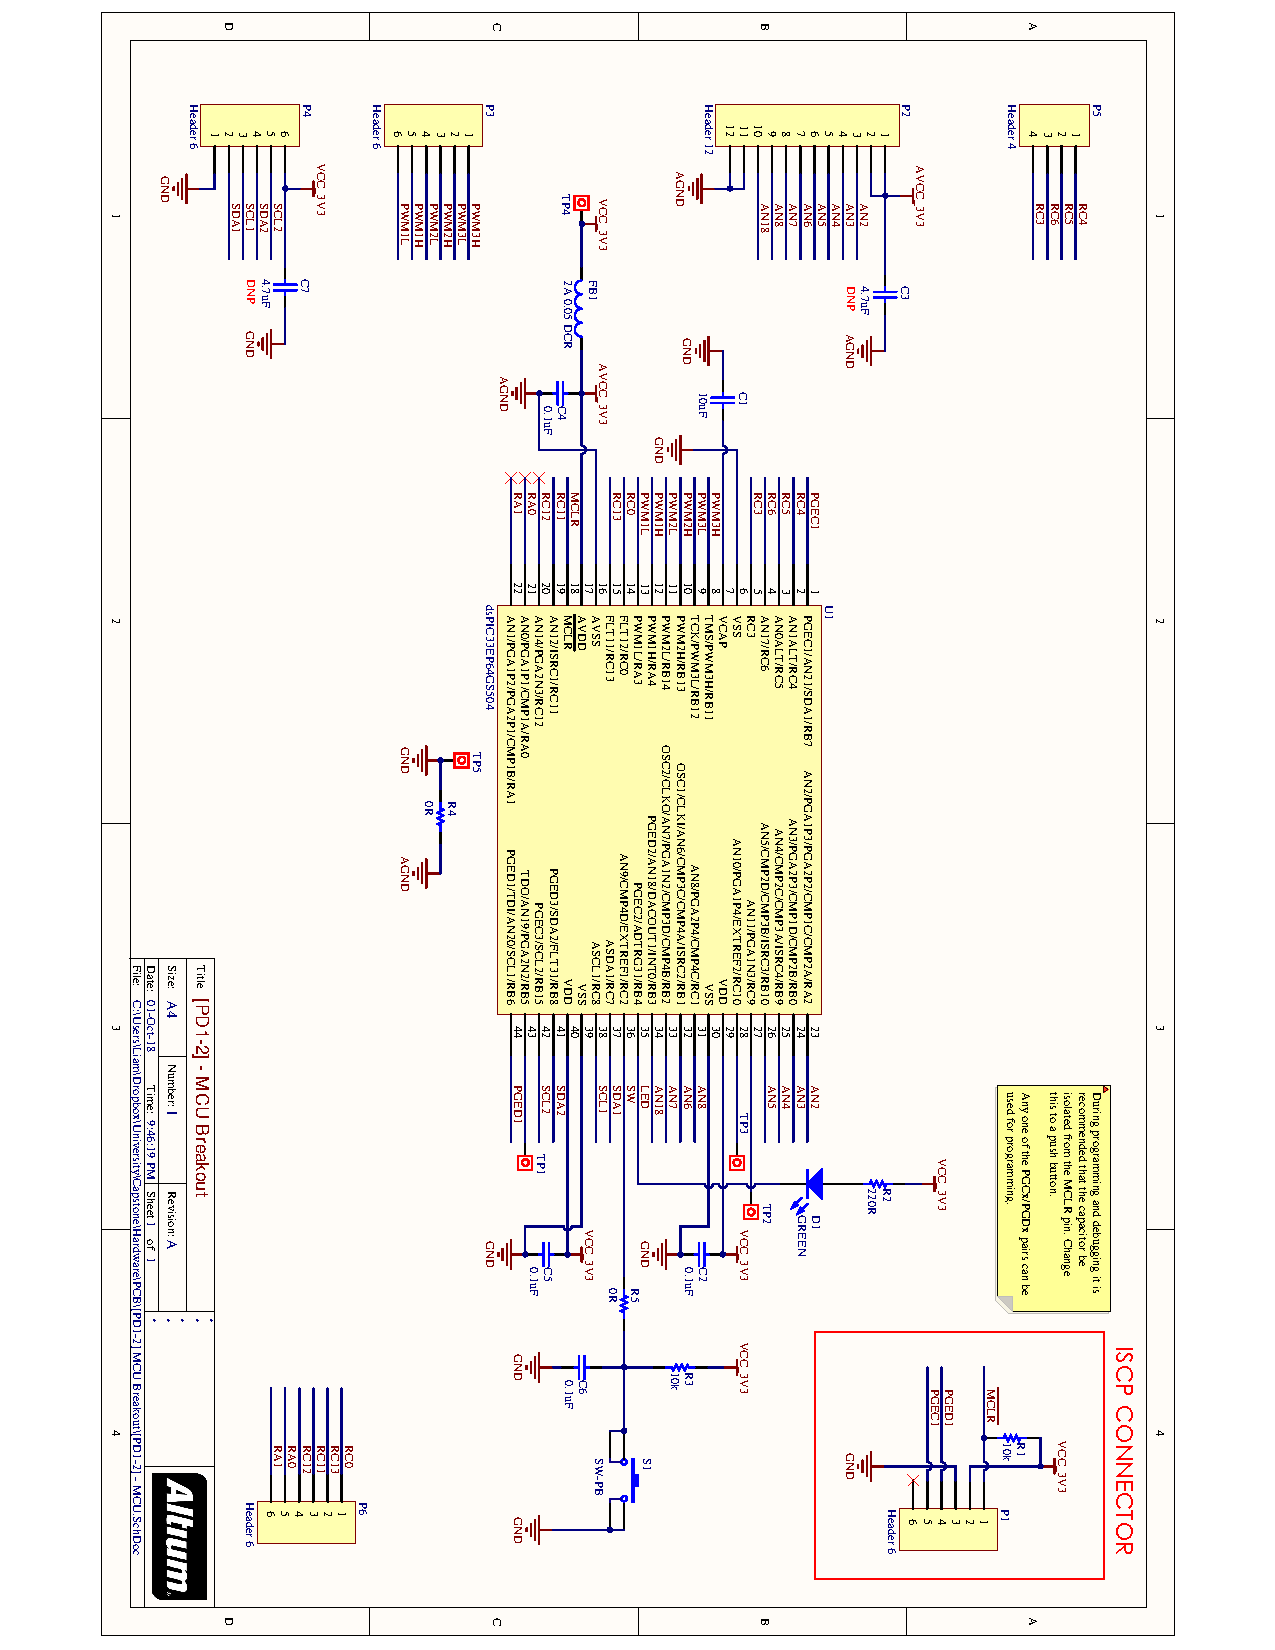
\includepdf[pages=-]{mcu_breakout.pdf}
\subsection{Controller and ultra-capacitor charging}
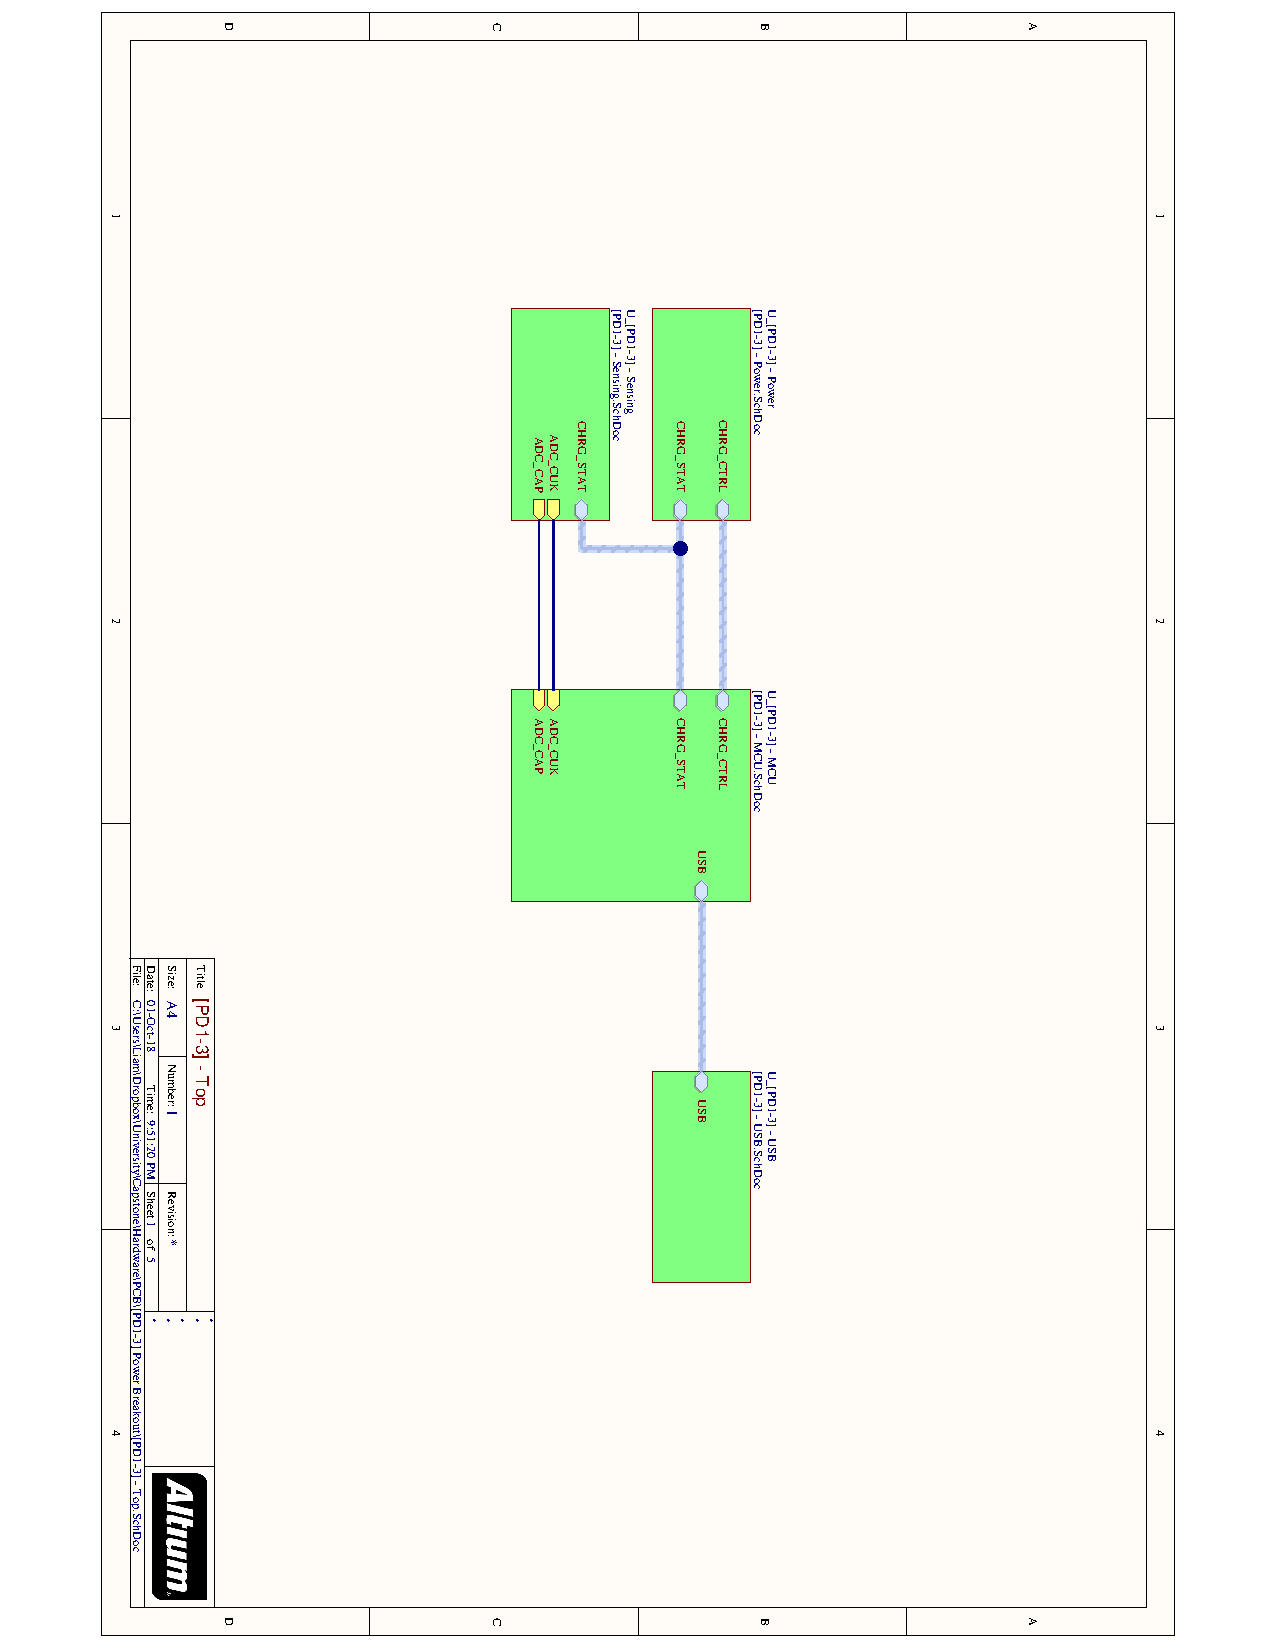
\includepdf[pages=-]{power_breakout.pdf}
\subsection{\'Cuk converter and driving}
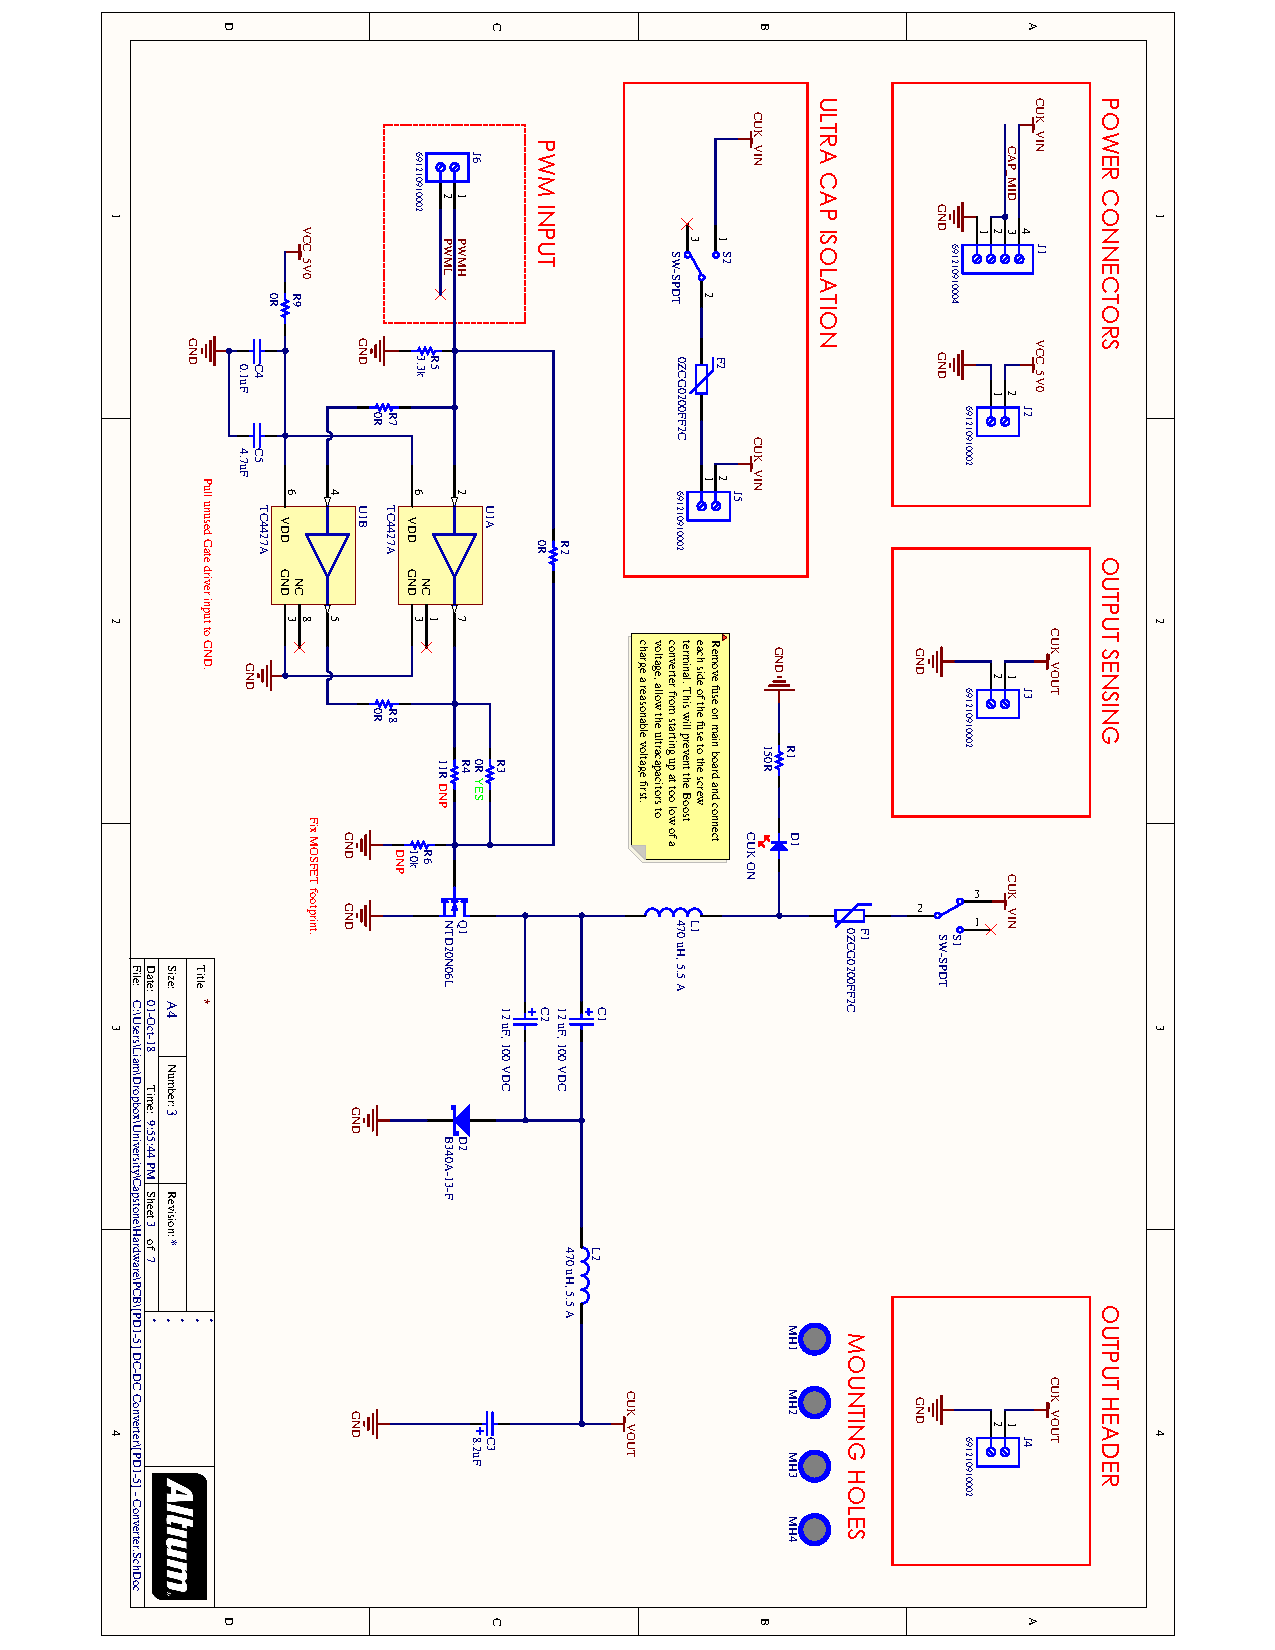
\includepdf[pages=-]{converter.pdf}
%%%%%%%%%%%%%%%%%%%%%%%%%%%%%%%%%%%%%%%%%%%%%%%%%%%%%%%%%%%%%%%%%%%%%%%%%%%%%%%%
%%%%%%%%%%%%%%%%%%%%%%%%%%%%%%%%%%%%%%%%%%%%%%%%%%%%%%%%%%%%%%%%%%%%%%%%%%%%%%%%
\newpage
%%%%%%%%%%%%%%%%%%%%%%%%%%%%%%%%%%%%%%%%%%%%%%%%%%%%%%%%%%%%%%%%%%%%%%%%%%%%%%%%
\section{Simulations}
% \subsection{Anti-Aliasing Filter}
\subsection{MOSFET Gate Driver} \label{apx:sim_mosfet}
Using LTSpice the chosen MOSFET for the \'Cuk Converter hardware implementation was modelled to determine the theoretical maximum current draw for the \SI{100}{kHz} switching frequency. The circuit shown in figure \ref{fig:sim_mosfet_circuit}.
\begin{figure}[H]
    \centering
    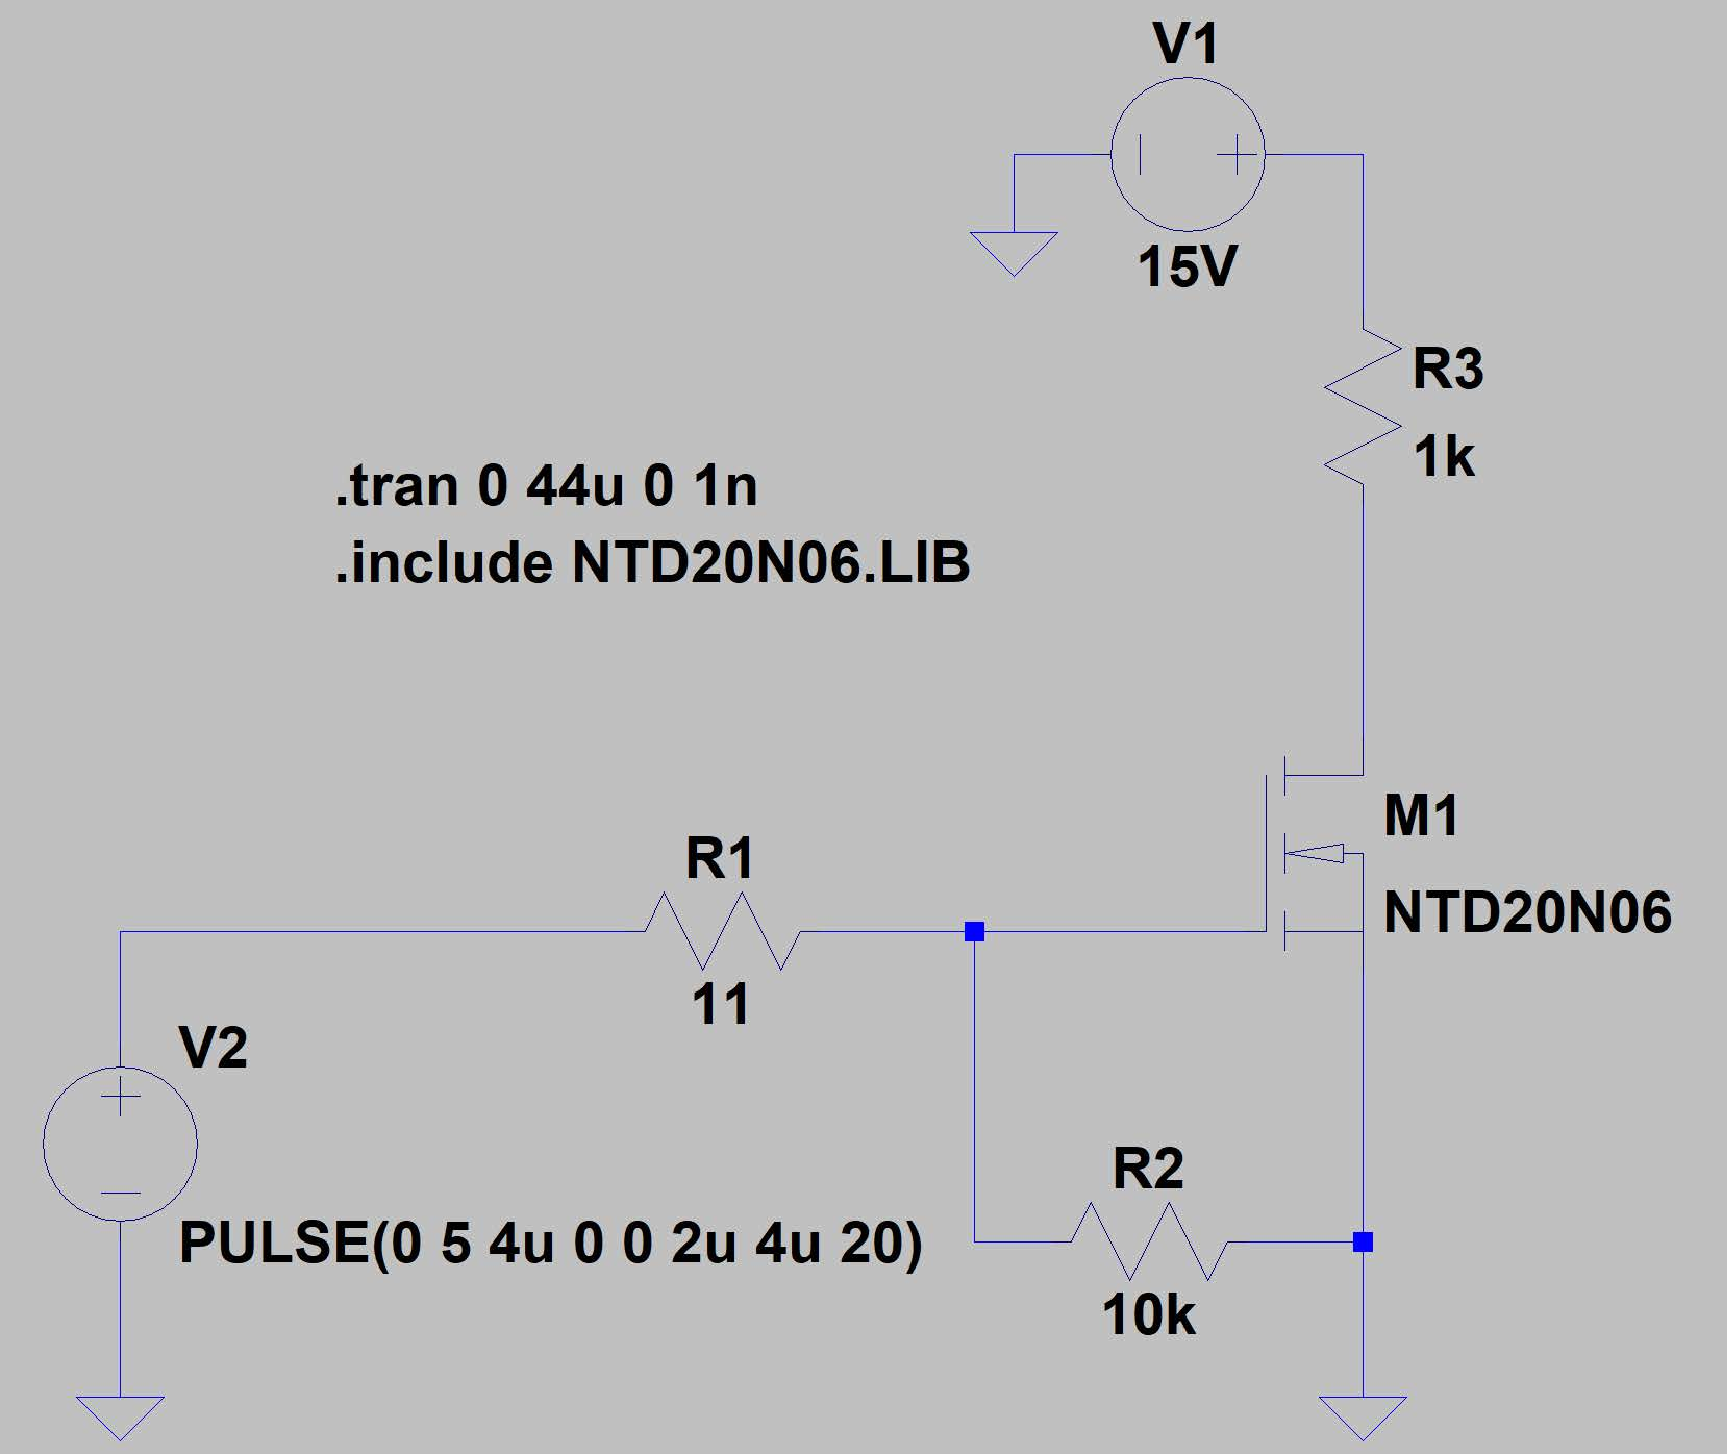
\includegraphics[width = \textwidth]{figures/appendix/sim_mosfet_gate.pdf}
    \caption{MOSFET gate driver simulation circuit.}
    \label{fig:sim_mosfet_circuit}
\end{figure}
Through experimentation the current limiting resistance $R_1$ was varied and found that \SI{10}{\ohm} gave a good compromise between switching speed and current. Despite this the gate current can reach $\pm\SI{180}{mA}$ which well exceeds the input/output source/sink of the microcontroller. This is shown in figure \ref{fig:sim_mosfet_plot}.
\begin{figure}[H]
    \centering
    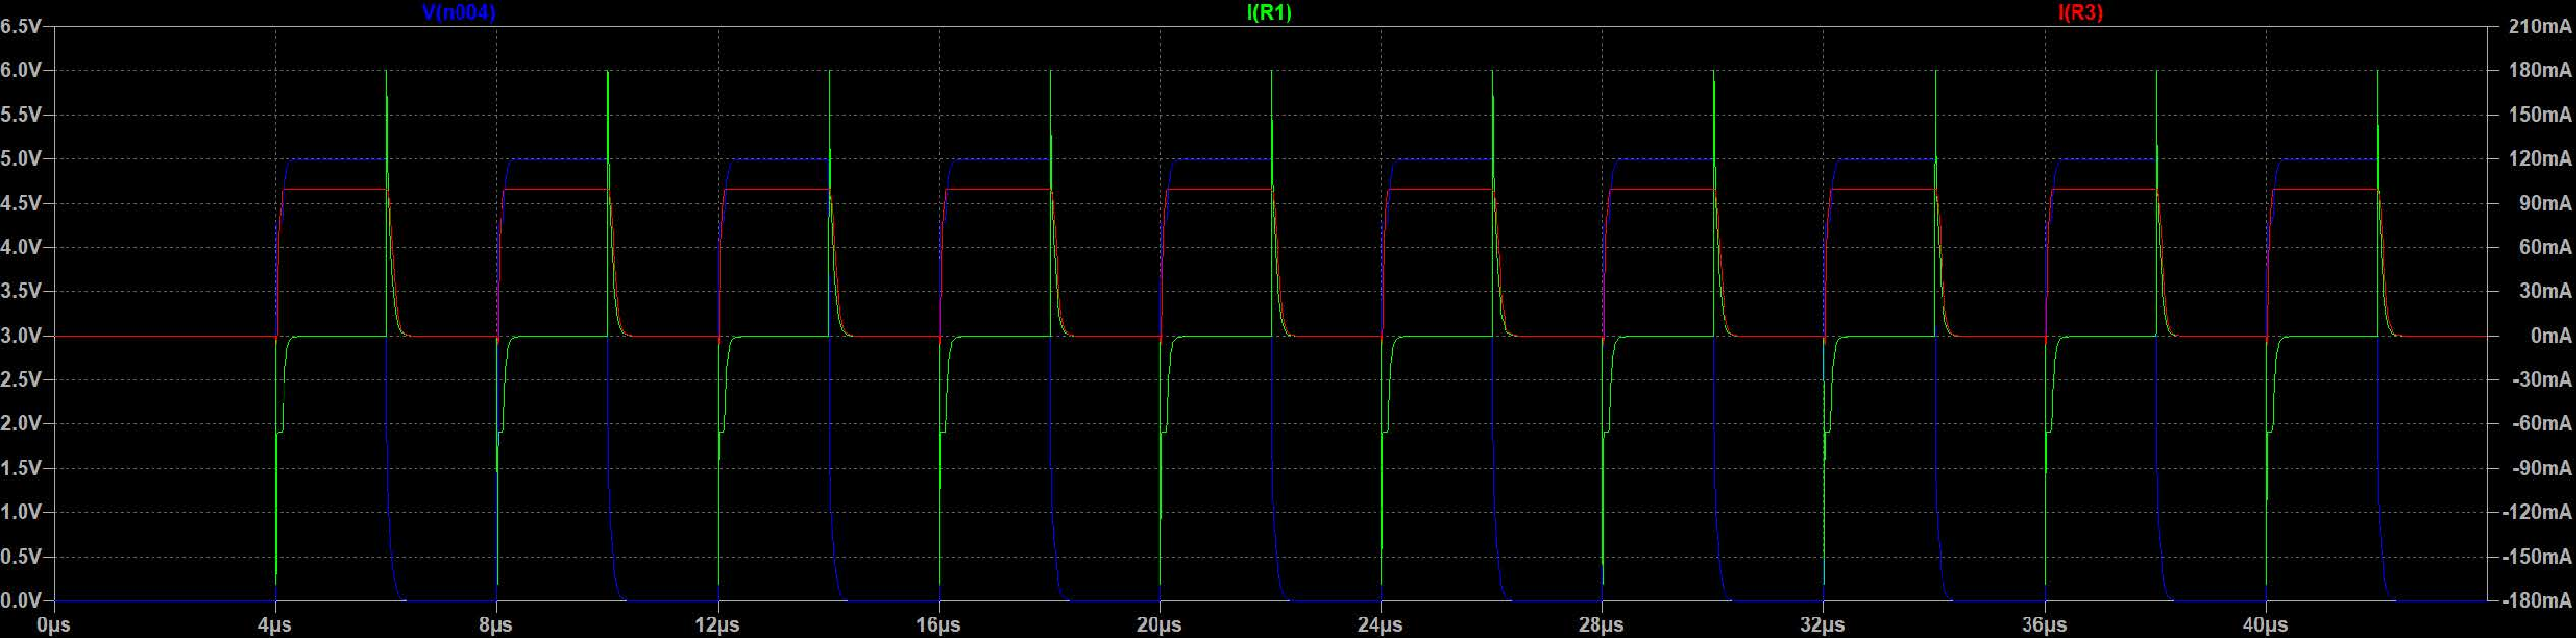
\includegraphics[width = \textwidth]{figures/appendix/sim_mosfet_gate_plot.pdf}
    \caption{MOSFET gate driver simulation plot.}
    \label{fig:sim_mosfet_plot}
\end{figure}
\subsection{\textsf{MATLAB} script}\label{apx:MATLAB}
Used in conjunction with the \textsf{Simulink} model of Figure~\ref{fig:simulink}.
\lstinputlisting{script_MATLAB.m}
%%%%%%%%%%%%%%%%%%%%%%%%%%%%%%%%%%%%%%%%%%%%%%%%%%%%%%%%%%%%%%%%%%%%%%%%%%%%%%%%
%%%%%%%%%%%%%%%%%%%%%%%%%%%%%%%%%%%%%%%%%%%%%%%%%%%%%%%%%%%%%%%%%%%%%%%%%%%%%%%%
%%%%%%%%%%%%%%%%%%%%%%%%%%%%%%%%%%%%%%%%%%%%%%%%%%%%%%%%%%%%%%%%%%%%%%%%%%%%%%%%
\clearpage
\section{Bill of Materials}
\begin{figure}[H]
    \centering
    \fbox{
    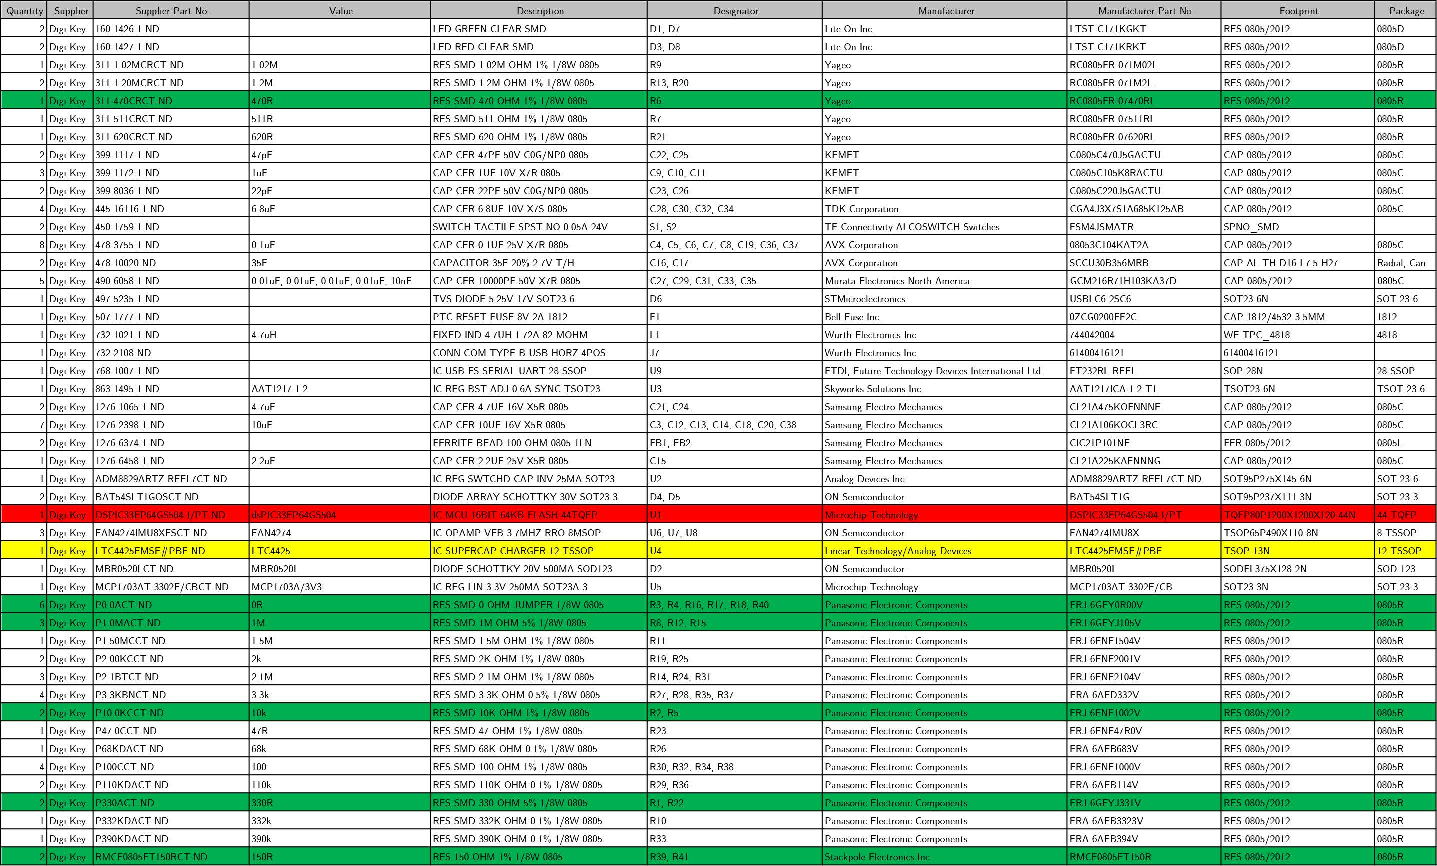
\includegraphics[angle=90, origin=c, height = \textwidth]{figures/BOM.pdf}
    }
    %\caption{}
    \label{}
\end{figure}
%%%%%%%%%%%%%%%%%%%%%%%%%%%%%%%%%%%%%%%%%%%%%%%%%%%%%%%%%%%%%%%%%%%%%%%%%%%%%%%%
%%%%%%%%%%%%%%%%%%%%%%%%%%%%%%%%%%%%%%%%%%%%%%%%%%%%%%%%%%%%%%%%%%%%%%%%%%%%%%%%
%%%%%%%%%%%%%%%%%%%%%%%%%%%%%%%%%%%%%%%%%%%%%%%%%%%%%%%%%%%%%%%%%%%%%%%%%%%%%%%%
\clearpage
\section{Microcontroller code}
\subsection{main}
\lstinputlisting[language=C]{MCUcode/main.c}

\subsection{Controller}
\lstinputlisting[language=C]{MCUcode/controller.c}

\subsection{myConversion}
\lstinputlisting[language=C]{MCUcode/myConversion.c}

\subsection{ADC}
\lstinputlisting[language=C]{MCUcode/adc.c}

\subsection{PWM}
\lstinputlisting[language=C]{MCUcode/pwm.c}

\subsection{Timer}
\lstinputlisting[language=C]{MCUcode/timer.c}

\subsection{UART}
\lstinputlisting[language=C]{MCUcode/uart.c}


%%%%%%%%%%%%%%%%%%%%%%%%%%%%%%%%%%%%%%%%%%%%%%%%%%%%%%%%%%%%%%%%%%%%%%%%%%%%%%%%
%%%%%%%%%%%%%%%%%%%%%%%%%%%%%%%%%%%%%%%%%%%%%%%%%%%%%%%%%%%%%%%%%%%%%%%%%%%%%%%%
%%%%%%%%%%%%%%%%%%%%%%%%%%%%%%%%%%%%%%%%%%%%%%%%%%%%%%%%%%%%%%%%%%%%%%%%%%%%%%%%